%    Template for seminar reports
% Seminar Current Topics in Computer Vision and Machine Learning
% Summer Semester 2015
% Computer Vision Group, Visual Computing Institute, RWTH Aachen

\documentclass[twoside,a4paper,article]{combine}


% =========================================================================
\usepackage[utf8]{inputenc}
\usepackage[ngerman]{babel}
\usepackage{a4}
\usepackage{fancyhdr}   
%\usepackage{german}    % Uncomment this iff you're writing the report in German
\usepackage{makeidx}
\usepackage{color}
\usepackage{t1enc}		% german letters in the "\hyphenation" - command
\usepackage{latexsym}	% math symbols
\usepackage{amssymb}    % AMS symbol fonts for LaTeX.

\usepackage{graphicx}
\usepackage{pslatex}
\usepackage{ifthen}

\usepackage[T1]{fontenc}
\usepackage{pslatex}

\usepackage{psfrag}
\usepackage{subfigure}
\usepackage{url}

% =========================================================================

\setlength{\oddsidemargin}{3.6pt}
\setlength{\evensidemargin}{22.6pt}
\setlength{\textwidth}{426.8pt}
\setlength{\textheight}{654.4pt}
\setlength{\headsep}{18pt}
\setlength{\headheight}{15pt}
\setlength{\topmargin}{-41.7pt}
\setlength{\topskip}{10pt}
\setlength{\footskip}{42pt}

\setlength{\parindent}{0pt}

% =========================================================================

\graphicspath{
	{img/}
}

%%%
% We want also subsubsections to be enumerated
%%%
\setcounter{secnumdepth}{3}
\setcounter{tocdepth}{3}

\makeglossary
%\makeindex

% =========================================================================
\begin{document}

% Template for seminar reports
% Seminar Current Topics in Computer Vision and Machine Learning

\begin{titlepage}


\begin{center}
\ 
\vspace{3.5cm}


\textsf
{
Fakultät für Mathematik, Informatik und Naturwissenschaften\\
Lehr- und Forschungsgebiet Informatik VIII\\
Computer Vision\\
Prof. Dr. Bastian Leibe
}

\rule{\linewidth}{1pt}

\vspace{1.75cm}
\LARGE
\textbf{Seminar Report}

\vspace{1.7cm}
\huge
Combining 3D Shape, Color, and Motion for Robust Anytime Tracking

\vspace{3.0cm}
\Large
Frederik Zwilling\\
\large
Matriculation Number: 304314

\vspace{0.5cm}
June 2015

\vspace{1.05cm}
\rule{\linewidth}{1pt}

\vspace{0.5cm}
\textsf{\textbf{
\normalsize
\begin{tabular}{ll}
Advisor:  & Aljoša Ošep\\
\end{tabular}
}}
\end{center}

\end{titlepage}


\begin{abstract}
  \textcolor{red}{Abstract}
\end{abstract}

\tableofcontents
\newpage
% =========================================================================

\section{Introduction}
\label{sec:intro}
Robust and precise position and velocity estimation is an important
part of object tracking. It is an essential part in the collision
avaidance of an autonomous car, for example. This report presents a
method by Held, Levinson, Thrun, and Savarese to solve this part of
the tracking problem by combining the 3D shape, color and motion of
the tracked object~\cite{paper}. The method uses a probabilistic
measurement model in form of a Dynamic Bayesian Network. The state
space of position and velocity for each tracked object is represented
in a special dynamic histogram, called \textit{annealed dynamic
  histogram}. This histogram dynamically increases its resolution in
the important areas and considers the local resolution in the
measurement model. By expanding the measurement model with color the
method results can be further improved. This is shown by the authors
by evaluating in a static environment where only the reference system
is moving and in a dynamic environment where the compactness of the
models build with the tracking results is used as evaluation criteria. 


\subsection{Motivation}
\label{sub:motivation}
Robotic applications are about to change many domains from the ground
up. Especially autonomous systems could take over dangerous,
exhausting and unpopular tasks and allow humans to do more satisfying
tasks instead. Additionally, autonomous systems can be more efficient
and scalable than solving the tasks by hand. Some progressive domains
with autonomous robots are flying drones, which can map
areas~\cite{auto-drones} or deliver
packages~\cite{auto-delivery-drones}, autonomous cars, which take care
of driving~\cite{auto-cars}, logistic robots, which store and grab
goods in warehouses~\cite{kiva}, and domestic service robots, which
can support old people and clean at home~\cite{athome}. All these
domains have in common that the robots have to track objects in their
environment, mostly for avoiding collisions, in the case of domestic
service robot also to follow people for example. Often the reliability
and precision of the tracking are limiting factors. An autonomous car,
for example, can only drive fast if it is absolutely sure that it
tracks all objects in the sorounding correctly and none of these
objects could cause a collision.  This report mainly focuses on the
domain of autonomous cars. Here, the autonomous system takes care of
the time consuming driving task on the one hand and could help to
reduce the amount of traffic deaths ($25,938$ in $2013$ in the
EU~\cite{traffic-deaths}) on the other hand. In this domain it is
especially important to estimate the speed of various nearby objects
robustly and in real time. Figure~\ref{fig:objects} shows the three
main classes of objects that have to be tracked, cars, bicycles, and
pedestrians, in challenging situations. The method proposed in this
report solves this task and performs better than previous approaches
in the car domain.
\begin{figure}
  \label{fig:objects}
  \subfigure[Cars on a highway]{%
    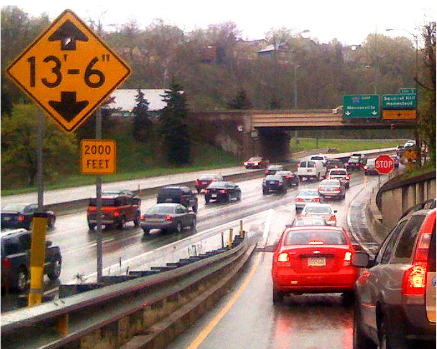
\includegraphics[height=.3\linewidth]{highway}
  }
  \subfigure[A cyclist]{%
    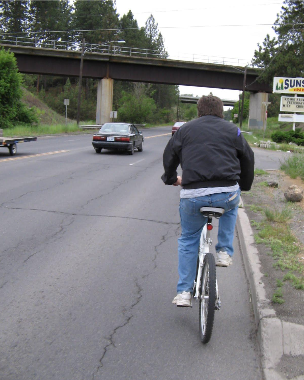
\includegraphics[height=.3\linewidth]{bicycle}
  }
  \subfigure[A pedestrian]{%
    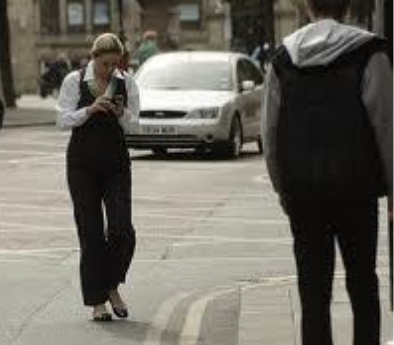
\includegraphics[height=.3\linewidth]{pedestrian}
  }
  
  \caption{Various objects that have to be tracked in challenging
    situations~\cite{held-website}}
\end{figure}


\subsection{Tracking}
\label{sub:tracking}
Object tracking is the complex task to identify objects and their
movement over time. It can be seperated into the following parts. The
first step segments the sensor data for time $t$, called
\textit{frame}, into detected objects. This can be done for example by
seperating foreground and background and find connected components in
the foreground. In this step it is benificial to use that
the most important objects to find are cars, bicycles and
pedestrians~\cite{segmentation}. The second step is to associate
detected object in the successive frames $t$ and $t+1$. One method to
find these matchings is to compute descriptors, such as the HOG
descriptor, for the objects and find nearest neighbors in the
descriptor space~\cite{arbitrary-object-recognition}. The third step
is the position and velocity estimation of the tracked object. That is
the part of tracking this report is about.

The data that is used for tracking in this report is generated by a
dense laser sensor that measures the distance to sourounding objects
with multiple rotating laser beams. Such a sensor and the data
generated by it is shown in Figure~\ref{fig:lidar}. Additionally, the
sensor provides a camera image similar to a panorama.
\begin{figure}
  \label{fig:lidar}
  \center
  \subfigure[]{%
    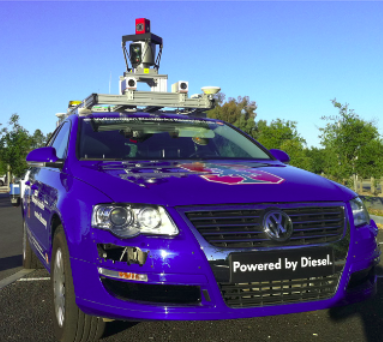
\includegraphics[height=.35\linewidth]{lidar}
  }
  \subfigure[]{%
    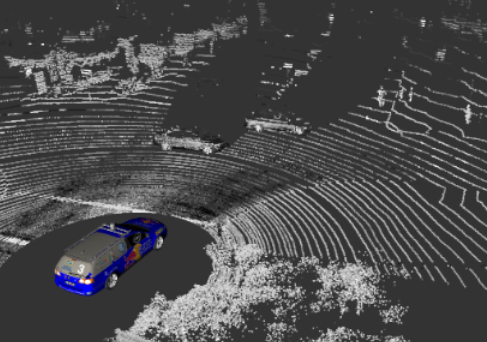
\includegraphics[height=.35\linewidth]{lidar-data}
  }
  
  \caption{A Velodyne LIDAR sensor mounted on a car (a) and a
    visualizaiton of the point cloud generated by it
    (b)~\cite{arbitrary-object-recognition}}
\end{figure}

\subsection{Velocity and Pose Estimation}
\label{sub:vel-and-pos-estimation}
To compute the pose and velocity estimation of an object, we first
introduce a measurement model that is derived from a Dynamic Bayesian
Network (\textit{DBN}). This DBN models for each frame the
dependencies between position, velocity, object surface and the
observed measurement as well as the dependencies between two
frames. This model uses shape and motion. Though tracking is a hard
problem because in cases with occlusion and major changes in the
viewpoint the visible object surface can differ significantly and
introduce an error. Especially in these cases, it is intuitive to also
consider color in the measurement model because the additional
information is influenced less by occlusion and viewpoint changes.

To find the state, which is composed of position and velocity of an
object, we use a histogram that maps the each histogram-chunk in the
state space to the probability that this chunk causes the measurement
according to our model. This allows a global search in the state space
with multiple hypothesis. A standard histogram with adequate
resolution would have to many chunks and thus would be to slow for
real time computation. Therefore, we use a dynamic histogram that
starts with a low resolution and an approximated posterior
distribution. Thenit dynamically increases the resolution in areas
with high probability to cause the measurement. This allows to achive
a result after running the method for any time. The downside of the
dynamic histogram is that the initial low resolution introduces an
additional error. This can be balanced by including the resolution in
the measurement model. We call this method \textit{annealed dynamic
  histogram} because as the resolution increases, the distribution is
annealed and approaches the true posterior.

The evaluation in Section~\ref{sec:evaluation} shows that the method
outperforms other tracking methods by about $10\%$.
\textcolor{red}{Maybe add more evaluation intro?}

% +++++++++++++++++++++++++
\section{Related Work}
\label{sec:related-work}
The tracking problem has been studied for many years. The most common
approaches to estimate the position and velocity of tracked objects,
namely Kalman filters and Iterative Closest Point,
are described in subsection~\ref{sub:pos-vel-est-alt}. Often these
approaches are efficient but sacrifice a lot of the available data by
using simple representations or search only for local maxima.
Because
our case of tracking objects in 3D point clouds from a laser sensor is
only a special case of tracking,
subsection~\ref{sub:slternative-sensors} gives an overview of the
tracking approaches with other sensors, mainly single cameras and
stereo cameras.
Subsection~\ref{sub:grid-based-methods} presents
grid-based approaches that are similar to annealed dynamic histograms.

\subsection{Position and velocity estimation alternatives}
\label{sub:pos-vel-est-alt}
A simple approach to estimate position and velocity of a tracked
object first represent the object by its
centroid~\cite{kalman-centroid, towards-aut-cars} or bounding
box~\cite{kalman-bounding-box, kalman-bounding-box2,
  kalman-bounding-box3} and then use a Kalman
filter~\cite{ai-modern}. This is a computationally efficient approach
but discards a lot of available information by using such a simple
representation. Therefore this approach is especially fragile in cases
of occlusion and viewpoint changes. In the occlusion case, the
bounding box can contain only a part of the object and the centroind
would be shifted. In the viewpoint-change case the centroid and
bounding box can significantly differ (e.g. when seeing a cyclist from
the back and the side). Another disadvantage of the Kalman filter is
that it can only represent a single hypothesis and thus performs
poorly when multiple hypotheses are reasonable.

Other approaches include domain specific knowledge to use better
fitting object representations. For example the typical shape of a car
with its corners or wheels could be use to achieve a more precise
position of an objet in a frame~\cite{use-car-shape, use-car-shape2,
  use-car-shape3}. This provides better detection and association
results but is limited by the amount of trained
object-classes. Although cars, pedestrians and cyclists are the most
common classes it is also important to detect uncommon obstacles in
traffic (e.g. tractors, segways, and wheelchairs). The work presented
in this report is based on~\cite{arbitrary-object-recognition}. It
allows recognition and classification of arbitrary objects and only
reuires a labled dataset to train the object-class.

A widely used alternative to Kalman filters is the Iterative Closest
Point (ICP) algorithm~\cite{icp, icp2}. The algorithm aligns merges
two point clouds by finding a maximum correspondence
alignment. Therefore the full 3D point cloud is used. It
uses a hill climbing approach and therefore depends on a good
initialization and can get stuck in local maxima. This is the major
limitation of ICP and has a large impact on the tracking precision as
shown by~\cite{icp-bad, icp-bad2}. Figure~\ref{fig:icp} visualizes how
ICP can return a wrong alignent after an unlucky initialization.
\begin{figure}
  \label{fig:icp}
  \center
  \subfigure[Bad initial alignment]{%
    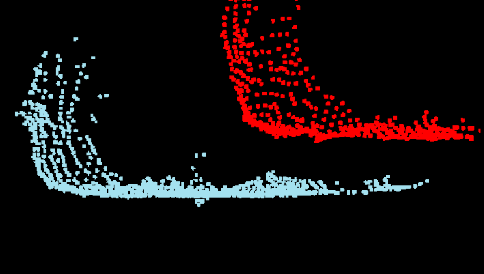
\includegraphics[height=.28\linewidth]{icp-init}
  }
  \subfigure[Stuck in a local maximum after 3 iterations
  (green arrows)]{%
    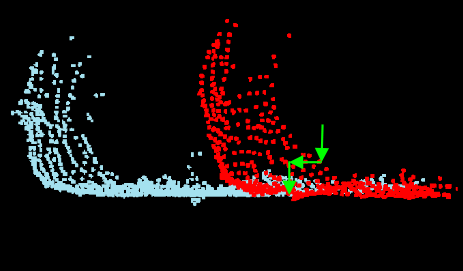
\includegraphics[height=.28\linewidth]{icp-stuck}
  }
  
  \caption{Possible case for bad ICP alignment results. The two point
    clouds belong a detected car in successive frames~\cite{held-website}.}
\end{figure}
The approach presented in this report performs a global search and
therefore has no problem with local maxima.

\subsection{Alternative Sensors}
\label{sub:slternative-sensors}

\subsection{Grid-Based Methods}
\label{sub:grid-based-methods}

% +++++++++++++++++++++++++
\section{Method}
\label{sec:method}
\subsection{Probabilistic Model}
\label{sub:probabilistic-model}
\subsection{Annealed Dynamic Histograms}
\label{sub:adh}
\subsection{Adding Color}
\label{sub:adding-color}

% +++++++++++++++++++++++++
\section{Evaluation}
\label{sec:evaluation}
\subsection{Relative Reference Frame}
\label{sub:relative-ref-frame}
\subsection{Model Crispness}
\label{sub:model-crispness}

% +++++++++++++++++++++++++
\section{Conclusion}
\label{sec:conclusion}


% =========================================================================
\bibliographystyle{alpha}
\bibliography{seminar_report}

% =========================================================================

\end{document}
